\documentclass{article}
\usepackage[a4paper, total={19cm, 26cm}]{geometry}
\usepackage[pdfusetitle]{hyperref}
\usepackage{url}
\usepackage{amssymb}
\usepackage{amsfonts}
\usepackage[backend=biber, style=alphabetic, sorting=none]{biblatex}
\addbibresource{main.bib}
\nocite{*}
\usepackage[usenames, dvipsnames, svgnames, x11names]{xcolor}
\usepackage{graphics}
\usepackage{scalerel}
\usepackage{accsupp}
\usepackage{stmaryrd}
\usepackage{listings}
\usepackage{lstcoq}
\usepackage{tikz}
\usetikzlibrary{positioning}
\usetikzlibrary{matrix}
\usetikzlibrary{bending}
\usetikzlibrary{arrows.meta}
\tikzstyle{node_matrix} = [matrix of nodes, nodes in empty cells, nodes = {anchor = center, minimum size = 20, draw, fill = blue!10, inner sep = 3.333}, inner sep = 0]
\tikzstyle{arrow} = [[-{>[length = 7, width = 5, bend]}]
\tikzstyle{leaf_tree_0} = [level distance = 25]
\tikzstyle{leaf_tree_1} = [level distance = 25, level 1/.style = {sibling distance = 20}]
\tikzstyle{leaf_tree_2} = [level distance = 25, level 1/.style = {sibling distance = 40}, level 2/.style = {sibling distance = 20}]
\tikzstyle{leaf_tree_3} = [level distance = 25, level 1/.style = {sibling distance = 80}, level 2/.style = {sibling distance = 40}, level 3/.style = {sibling distance = 20}]
\tikzstyle{leaf_tree_leaf} = [minimum size = 0, circle, draw]
\tikzstyle{leaf_tree_inner_node} = [minimum size = 0, circle, draw, inner sep = 1, fill = black]
\newcommand{\spacer}[0]{%
    \begin{tikzpicture}%
        \clip (0, 0) rectangle (0.001, 0.5);
    \end{tikzpicture}%
}
\newcommand{\bigvarnothing}[0]{%
    \scalebox{3}{%
        
\begin{tikzpicture}%
            \clip (-0.114, -0.1) rectangle (0.114, 0.128);
            \node [style = {inner sep = 0}, text = black!35] {$\varnothing$};
        \end{tikzpicture}%
    }%
}
\newcommand{\completebinaryleaftreedepthzero}[1]{%
    \begin{tikzpicture}%
        \begin{scope} [leaf_tree_0]
            \node [style = {leaf_tree_leaf}] {#1};
        \end{scope}
    \end{tikzpicture}%
}
\newcommand{\completebinaryleaftreedepthone}[2]{%
    \begin{tikzpicture}%
        \begin{scope} [leaf_tree_1]
            \node [style = {leaf_tree_inner_node}] {}
                child {
                    node [style = {leaf_tree_leaf}] {#1}
                }
                child {
                    node [style = {leaf_tree_leaf}] {#2}
                };
        \end{scope}
    \end{tikzpicture}%
}
\newcommand{\completebinaryleaftreedepthtwo}[4]{%
    \begin{tikzpicture}%
        \begin{scope} [leaf_tree_2]
            \node [style = {leaf_tree_inner_node}] {}
                child {
                    node [style = {leaf_tree_inner_node}] {}
                    child {
                        node [style = {leaf_tree_leaf}] {#1}
                    }
                    child {
                        node [style = {leaf_tree_leaf}] {#2}
                    }
                }
                child {
                    node [style = {leaf_tree_inner_node}] {}
                    child {
                        node [style = {leaf_tree_leaf}] {#3}
                    }
                    child {
                        node [style = {leaf_tree_leaf}] {#4}
                    }
                };
        \end{scope}
    \end{tikzpicture}%
}
\newcommand{\completebinaryleaftreedepththree}[8]{%
    \begin{tikzpicture}%
        \begin{scope} [leaf_tree_3]
            \node [style = {leaf_tree_inner_node}] {}
                child {
                    node [style = {leaf_tree_inner_node}] {}
                    child {
                        node [style = {leaf_tree_inner_node}] {}
                        child {
                            node [style = {leaf_tree_leaf}] {#1}
                        }
                        child {
                            node [style = {leaf_tree_leaf}] {#2}
                        }
                    }
                    child {
                        node [style = {leaf_tree_inner_node}] {}
                        child {
                            node [style = {leaf_tree_leaf}] {#3}
                        }
                        child {
                            node [style = {leaf_tree_leaf}] {#4}
                        }
                    }
                }
                child {
                    node [style = {leaf_tree_inner_node}] {}
                    child {
                        node [style = {leaf_tree_inner_node}] {}
                        child {
                            node [style = {leaf_tree_leaf}] {#5}
                        }
                        child {
                            node [style = {leaf_tree_leaf}] {#6}
                        }
                    }
                    child {
                        node [style = {leaf_tree_inner_node}] {}
                        child {
                            node [style = {leaf_tree_leaf}] {#7}
                        }
                        child {
                            node [style = {leaf_tree_leaf}] {#8}
                        }
                    }
                };
        \end{scope}
    \end{tikzpicture}%
}
\newenvironment{no_space_center}
    {\parskip=0pt\par\nopagebreak\centering}
    {\par\noindent\ignorespacesafterend}
\newenvironment{no_padding_center}
    {\parskip=0pt\par\nopagebreak\centering}
    {\par\noindent}
\newcommand*{\llbrace}{%
    \BeginAccSupp{method=hex,unicode,ActualText=2983}%
    \textnormal{\usefont{OMS}{lmr}{m}{n}\char102}%
    \mathchoice{\mkern-4.05mu}{\mkern-4.05mu}{\mkern-4.3mu}{\mkern-4.8mu}%
    \textnormal{\usefont{OMS}{lmr}{m}{n}\char106}%
    \EndAccSupp{}%
}
\newcommand*{\rrbrace}{%
    \BeginAccSupp{method=hex,unicode,ActualText=2984}%
    \textnormal{\usefont{OMS}{lmr}{m}{n}\char106}%
    \mathchoice{\mkern-4.05mu}{\mkern-4.05mu}{\mkern-4.3mu}{\mkern-4.8mu}%
    \textnormal{\usefont{OMS}{lmr}{m}{n}\char103}%
    \EndAccSupp{}%
}
\newsavebox{\lXbrace}
\savebox{\lXbrace}{$\llbrace$}
\newsavebox{\rXbrace}
\savebox{\rXbrace}{$\rrbrace$}
\def\lxbrace{\scalerel*{\usebox{\lXbrace}}{\llbrace}}
\def\rxbrace{\scalerel*{\usebox{\rXbrace}}{\rrbrace}}
\newcommand{\xbraces}[1]{\scalerel[1.5ex]{\lxbrace}{#1}\scalerel*[1.5ex]{\rxbrace}{#1}}
\newcommand{\nospaceevaluatesto}[0]{\scaleobj{1.5}{\leadsto}}
\newcommand{\evaluatesto}[0]{\:\nospaceevaluatesto\:}
\title{Implementation and verification of a data structure using dependent types}
\author{Anton Danilkin}
\begin{document}

\begin{no_space_center}
    \begin{minipage}{10cm}
        \maketitle
    \end{minipage}
\end{no_space_center}

\begin{abstract}
    
\end{abstract}

\vspace{10cm}

\section{Introduction}

One of the most important data structures in functional programming are singly linked lists, which support prepending an element in the beginning, as well as destructing a non-empty list into its head (the first element) and tail (the list containing the rest of elements). Conversely, arrays are frequently used in imperative programming; they support getting and setting an element by its index, as well as, in case of vectors, dynamic resizing.

The problem of lists is that the operation of retrieving or updating an element at a specific index has linear spacial complexity in term of the size. On the flip side, operations on arrays and vectors mutate the instance they work on, which not only makes reasoning about program behavior harder, but also means that older versions of the data structure become unaccessible for future use. One way to fix that would be making a copy before each operation, but that again would mean that everything would have linear complexity.

For these reasons, the following question arises: is it possible to design a data structure that combines the benefits of singly linked lists and vectors?

\section{Similarities between numbers and lists}

Here are some standard definitions of Peano natural numbers and lists, as well as operations on them in Coq:

\begin{no_padding_center}
    \begin{tabular}{c c}
        \begin{coq}
Inductive nat :=
  | O : nat
  | S : nat -> nat.




Definition pred (n : nat) : nat :=
  match n with
  | O => O
  | S n' => n'
  end.

Fixpoint plus (n1 n2 : nat) : nat :=
  match n1 with
  | O => n2
  | S n1' => S (plus n1' n2)
  end.
        \end{coq} &
        \begin{coq}
Inductive list A :=
  | nil : list A
  | cons : A -> list A -> list A.

Arguments nil {A}.
Arguments cons {A} x l.

Definition tl {A} (l : list A) : list A :=
  match l with
  | nil => nil
  | cons _ l' => l'
  end.

Fixpoint app {A} (l1 l2 : list A) : list A :=
  match l1 with
  | nil => l2
  | cons x l1' => cons x (app l1' l2)
  end.
        \end{coq}
    \end{tabular}
\end{no_padding_center}

As remarked by Chris Okasaki \cite{okasaki_1998}, there is a clear resemblance between them: the only real difference is that \coqinline{list A} holds a datum of type \coqinline{A}, where as \coqinline{nat} does not. Here is how the list \coqinline{[7; 5; 8]} and the number 3 (which is the length of the list) could be represented:

\begin{center}
    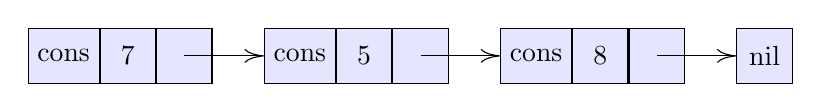
\begin{tikzpicture}
        \matrix (node1) [node_matrix, anchor = west] at (0, 0) {
            \coqinlinelight{cons} &
            7 &
            \\
        };
        \matrix (node2) [node_matrix, anchor = west] at (3, 0) {
            \coqinlinelight{cons} &
            5 &
            \\
        };
        \matrix (node3) [node_matrix, anchor = west] at (6, 0) {
            \coqinlinelight{cons} &
            8 &
            \\
        };
        \matrix (node4) [node_matrix, anchor = west] at (9, 0) {
            \coqinlinelight{nil} \\
        };
        \draw [arrow] (node1-1-3.center) to (node2-1-1);
        \draw [arrow] (node2-1-3.center) to (node3-1-1);
        \draw [arrow] (node3-1-3.center) to (node4-1-1);
    \end{tikzpicture}
\end{center}

\begin{center}
    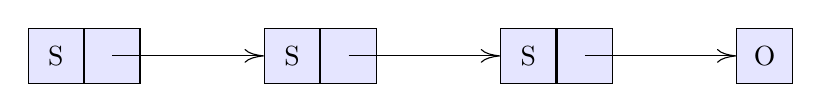
\begin{tikzpicture}
        \matrix (node1) [node_matrix, anchor = west] at (0, 0) {
            \coqinlinelight{S} &
            \\
        };
        \matrix (node2) [node_matrix, anchor = west] at (3, 0) {
            \coqinlinelight{S} &
            \\
        };
        \matrix (node3) [node_matrix, anchor = west] at (6, 0) {
            \coqinlinelight{S} &
            \\
        };
        \matrix (node4) [node_matrix, anchor = west] at (9, 0) {
            \coqinlinelight{O} \\
        };
        \draw [arrow] (node1-1-2.center) to (node2-1-1);
        \draw [arrow] (node2-1-2.center) to (node3-1-1);
        \draw [arrow] (node3-1-2.center) to (node4-1-1);
    \end{tikzpicture}
\end{center}

In fact, we can go from a list to the corresponding natural number by getting its length, and back from a natural number to one of the corresponding lists by repeating an element that many times:

\begin{no_padding_center}
    \begin{tabular}{c c}
        \begin{coq}
Fixpoint length {A} (l : list A) : nat :=
  match l with
  | nil => O
  | cons _ l' => S (length l')
  end.
        \end{coq} &
        \begin{coq}
Fixpoint repeat {A} (x : A) (n : nat) : list A :=
  match n with
  | O => nil
  | S n' => cons x (repeat x n')
  end.
        \end{coq}
    \end{tabular}
\end{no_padding_center}

\section{Binary non-dependent version}

As there are many ways to represent natural numbers (and not only the unary system that was considered above). Depending on which representation we chose, operations on the numbers (such as increment, decrement, sum, converting into other representations) will have different efficiency, and in each case we can find an analogous data structure.

So another simple representation of natural numbers is the binary numeral system. As seen, again, by Chris Okasaki \cite{okasaki_1998}, we can augment it to contain pieces of data by complete binary leaf trees in each digit of the number (although here we will use big-endian digit ordering instead of little-endian).

For the following, we will denote by \coqinline{A} some data type (in examples in will be \coqinline{nat}). A ``complete binary leaf tree'' of depth $d$ has $2^d$ leaves where it stores values of type \coqinline{A} (``complete binary'' meaning that each internal node has exactly 2 children, ``leaf'' meaning that data is only stores in the leaves).

\begin{coq}
Inductive binary_leaf_tree {A} :=
  | BinaryLeafTreeLeaf : A -> binary_leaf_tree
  | BinaryLeafTreeInternalNode : binary_leaf_tree -> binary_leaf_tree -> binary_leaf_tree.

Arguments binary_leaf_tree : clear implicits.
\end{coq}

Here is an example of a complete binary leaf tree of depth $2$ holding values $0$, $1$, $2$, $3$:

\begin{center}
    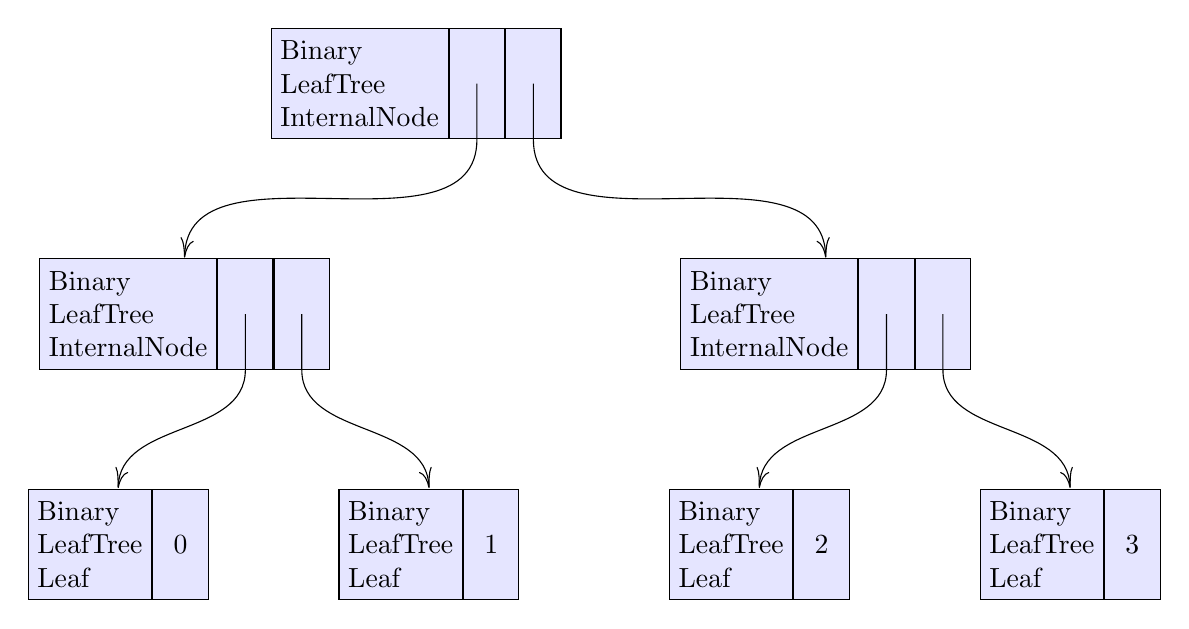
\begin{tikzpicture}
        \matrix (node1) [node_matrix, nodes = {minimum height = 40}, anchor = center] {
            \node (node1-1-1) [align = left] {\coqinlinelight{Binary} \\ \coqinlinelight{LeafTree} \\ \coqinlinelight{InternalNode}}; &
            &
            \\
        };
        \matrix (node2) [node_matrix, nodes = {minimum height = 40}, anchor = center, node distance = 1.5 and 1.5, below left = of node1-1-2] {
            \node (node2-1-1) [align = left] {\coqinlinelight{Binary} \\ \coqinlinelight{LeafTree} \\ \coqinlinelight{InternalNode}}; &
            &
            \\
        };
        \matrix (node3) [node_matrix, nodes = {minimum height = 40}, anchor = center, node distance = 1.5 and 1.5, below right = of node1-1-3] {
            \node (node3-1-1) [align = left] {\coqinlinelight{Binary} \\ \coqinlinelight{LeafTree} \\ \coqinlinelight{InternalNode}}; &
            &
            \\
        };
        \matrix (node4) [node_matrix, nodes = {minimum height = 40}, anchor = center, node distance = 1.5 and 0.1, below left = of node2-1-2] {
            \node (node4-1-1) [align = left] {\coqinlinelight{Binary} \\ \coqinlinelight{LeafTree} \\ \coqinlinelight{Leaf}}; &
            $0$ \\
        };
        \matrix (node5) [node_matrix, nodes = {minimum height = 40}, anchor = center, node distance = 1.5 and 0.1, below right = of node2-1-3] {
            \node (node5-1-1) [align = left] {\coqinlinelight{Binary} \\ \coqinlinelight{LeafTree} \\ \coqinlinelight{Leaf}}; &
            $1$ \\
        };
        \matrix (node6) [node_matrix, nodes = {minimum height = 40}, anchor = center, node distance = 1.5 and 0.1, below left = of node3-1-2] {
            \node (node6-1-1) [align = left] {\coqinlinelight{Binary} \\ \coqinlinelight{LeafTree} \\ \coqinlinelight{Leaf}}; &
            $2$ \\
        };
        \matrix (node7) [node_matrix, nodes = {minimum height = 40}, anchor = center, node distance = 1.5 and 0.1, below right = of node3-1-3] {
            \node (node7-1-1) [align = left] {\coqinlinelight{Binary} \\ \coqinlinelight{LeafTree} \\ \coqinlinelight{Leaf}}; &
            $3$ \\
        };
        \draw [arrow] (node1-1-2.center) -- (node1-1-2.south) to[out = -90, in = 90] (node2.north);
        \draw [arrow] (node1-1-3.center) -- (node1-1-3.south) to[out = -90, in = 90] (node3.north);
        \draw [arrow] (node2-1-2.center) -- (node2-1-2.south) to[out = -90, in = 90] (node4.north);
        \draw [arrow] (node2-1-3.center) -- (node2-1-3.south) to[out = -90, in = 90] (node5.north);
        \draw [arrow] (node3-1-2.center) -- (node3-1-2.south) to[out = -90, in = 90] (node6.north);
        \draw [arrow] (node3-1-3.center) -- (node3-1-3.south) to[out = -90, in = 90] (node7.north);
    \end{tikzpicture}
\end{center}

They will be drawn like that in the future:

\begin{center}
    \completebinaryleaftreedepthtwo{$0$}{$1$}{$2$}{$3$}
\end{center}

We know that for each natural number $n$ there are $d \in \mathbb{N}$ and $n_{d - 1}, n_{d - 2}, ..., n_0, n_1 \in \{0, 1\}$ such that $n = n_{d - 1} 2^{d - 1} + n_{d - 2} 2^{d - 2} + ... + n_1 2^1 + n_0 2^0$. The function \coqinline{to_digits : forall (d n : nat), list nat} gives the list of length \coqinline{d} consisting of these binary digits of \coqinline{n} in big-endian ordering: for example, \coqinline{to_digits 8 73 ~> [0; 1; 0; 0; 1; 0; 0; 1]} (where ``\nospaceevaluatesto'' means ``evaluates to''). The inverse operation is \coqinline{of_digits : forall (d : nat) (nl : list nat), nat}: for example, \coqinline{of_digits 8 [0; 1; 0; 0; 1; 0; 0; 1] ~> 73}.

A ``digital list'' of depth $d$ is a list of length $d$ of which the $k$'th element is a complete binary leaf tree of depth $k$ if $n_k = 1$ and nothing otherwise.

\begin{coq}
Inductive digital_list {A} :=
  | DigitalListNil : digital_list
  | DigitalListCons : option (binary_leaf_tree A) -> digital_list -> digital_list.

Arguments digital_list : clear implicits.
\end{coq}

Here is an example of a digit list for $n = 5$, so $d = 3$, $n_2$ = 1, $n_1 = 0$, $n_2 = 1$, which stores values 0, 1, 2, 3, 4:

\begin{center}
    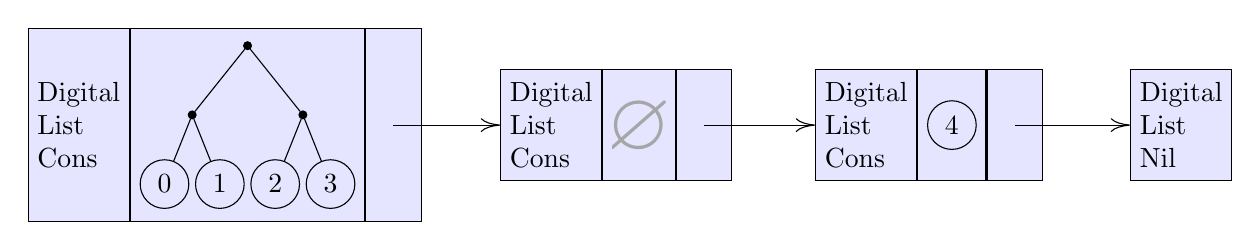
\begin{tikzpicture}
        \matrix (node1) [node_matrix, nodes = {minimum height = 70}, anchor = west] at (0, 0) {
            \node (node1-1-1) [align = left] {\coqinlinelight{Digital} \\ \coqinlinelight{List} \\ \coqinlinelight{Cons}}; &
            \completebinaryleaftreedepthtwo{$0$}{$1$}{$2$}{$3$} &
            \\
        };
        \matrix (node2) [node_matrix, nodes = {minimum height = 40}, anchor = west] at (6, 0) {
            \node (node2-1-1) [align = left] {\coqinlinelight{Digital} \\ \coqinlinelight{List} \\ \coqinlinelight{Cons}}; &
            \bigvarnothing &
            \\
        };
        \matrix (node3) [node_matrix, nodes = {minimum height = 40}, anchor = west] at (10, 0) {
            \node (node3-1-1) [align = left] {\coqinlinelight{Digital} \\ \coqinlinelight{List} \\ \coqinlinelight{Cons}}; &
            \completebinaryleaftreedepthzero{$4$} &
            \\
        };
        \matrix (node4) [node_matrix, nodes = {minimum height = 40}, anchor = west] at (14, 0) {
            \node (node4-1-1) [align = left] {\coqinlinelight{Digital} \\ \coqinlinelight{List} \\ \coqinlinelight{Nil}}; \\
        };
        \draw [arrow] (node1-1-3.center) to (node2-1-1);
        \draw [arrow] (node2-1-3.center) to (node3-1-1);
        \draw [arrow] (node3-1-3.center) to (node4-1-1);
    \end{tikzpicture}
\end{center}

Or, to simplify the drawing, the following notation will be used form now on:

\begin{center}
    $\xbraces{
        \vcenter{\hbox{\completebinaryleaftreedepthtwo{$0$}{$1$}{$2$}{$3$}}};
        \vcenter{\hbox{\bigvarnothing}};
        \vcenter{\hbox{\completebinaryleaftreedepthzero{$4$}}}
    }$
\end{center}

A ``concrete digital list'' is a $d \in \mathbb{N}$ and a digital list of depth $d$ (one of the reasons to store the depth explicitly is so that it can be accessed immediately).

\begin{coq}
Inductive concrete_digital_list {A} :=
  | ConcreteDigitalList : forall (d : nat), digital_list A -> concrete_digital_list.

Arguments concrete_digital_list : clear implicits.
\end{coq}

The following concrete digital list corresponds to the digital list given above:

\begin{center}
    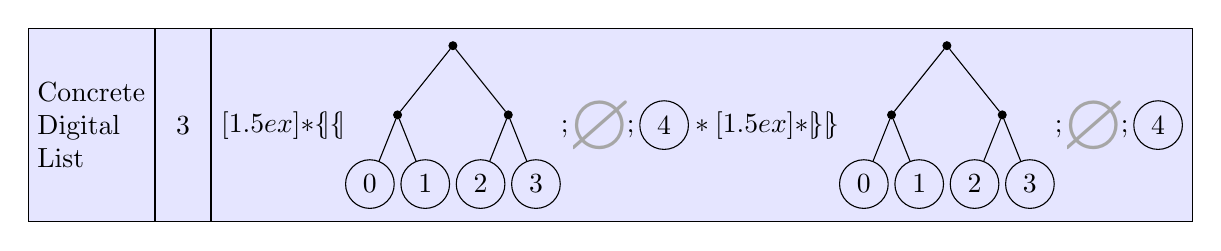
\begin{tikzpicture}
        \matrix (node1) [node_matrix, nodes = {minimum height = 70}, anchor = west] at (0, 0) {
            \node (node1-1-1) [align = left] {\coqinlinelight{Concrete} \\ \coqinlinelight{Digital} \\ \coqinlinelight{List}}; &
            $3$ &
            $\xbraces{
                \vcenter{\hbox{\completebinaryleaftreedepthtwo{$0$}{$1$}{$2$}{$3$}}};
                \vcenter{\hbox{\bigvarnothing}};
                \vcenter{\hbox{\completebinaryleaftreedepthzero{$4$}}}
            }$ \\
        };
    \end{tikzpicture}
\end{center}

Next we will consider operations that we can do with these types. We will first define each operation on binary leaf trees, then lift it to digital lists (always having a ``depth'' argument, which corresponds to the depth of the digital list passed, for consistency and for reasons outlined later, even when it is not actually used), and finally to concrete digital lists.

\subsection{Interpretation}

The first operation will be conversion to a simple list, which at the same times gives an ``interpretation'' of the data structures, allowing us to establish a convection between the operations on them and ones on the regular lists, which means proving the correctness of these operations.

To convert a binary leaf tree to a list, we just traverse its leaves in their natural order. For example:

\begin{center}
    \coqinline{binary_leaf_tree_to_list}
    $\vcenter{\hbox{\completebinaryleaftreedepthtwo{$0$}{$1$}{$2$}{$3$}}}$
    \coqinline{~> [0; 1; 2; 3]}
\end{center}

\begin{coq}
Fixpoint binary_leaf_tree_to_list {A} (blt : binary_leaf_tree A) :=
  match blt with
  | BinaryLeafTreeLeaf x => [x]
  | BinaryLeafTreeInternalNode blt'1 blt'2 =>
    binary_leaf_tree_to_list blt'1 ++ binary_leaf_tree_to_list blt'2
  end.
\end{coq}

For a digital list, we convert each binary leaf tree (if it exists) to a list and then concatenate the results. For example:

\begin{center}
    \coqinline{digital_list_to_list 3}
    $\xbraces{
        \vcenter{\hbox{\completebinaryleaftreedepthtwo{$0$}{$1$}{$2$}{$3$}}};
        \vcenter{\hbox{\bigvarnothing}};
        \vcenter{\hbox{\completebinaryleaftreedepthzero{$4$}}}
    }$
    \coqinline{~> [0; 1; 2; 3; 4]}
\end{center}

\begin{coq}
Fixpoint digital_list_to_list {A} d (dl : digital_list A) :=
  match dl with
  | DigitalListNil => []
  | DigitalListCons o dl' =>
    match o with
    | None => []
    | Some blt => binary_leaf_tree_to_list blt
    end ++ digital_list_to_list (pred d) dl'
  end.
\end{coq}

The version for concrete digital lists is straight-forward:

\begin{coq}
Definition concrete_digital_list_to_list {A} (cdl : concrete_digital_list A) :=
  let '(ConcreteDigitalList d dl) := cdl in digital_list_to_list d dl.
\end{coq}

\subsection{Length}

The length (the number of data elements stored) of a complete binary leaf tree of depth $d$ is, as remarked earlier, $2^d$. So to get the length of a digital list, we just sum the lengths of the binary leaf trees, at positions where they are present. For example:

\begin{center}
    \coqinline{digital_list_length 3}
    $\xbraces{
        \vcenter{\hbox{\completebinaryleaftreedepthtwo{$0$}{$1$}{$2$}{$3$}}};
        \vcenter{\hbox{\bigvarnothing}};
        \vcenter{\hbox{\completebinaryleaftreedepthzero{$4$}}}
    }$
    \coqinline{~> 5}
\end{center}

\begin{coq}
Fixpoint digital_list_length {A} d (dl : digital_list A) :=
  match dl with
  | DigitalListNil => 0
  | DigitalListCons o dl' => (if o then Nat.pow 2 (pred d) else 0) + digital_list_length (pred d) dl'
  end.

Definition concrete_digital_list_length {A} (cdl : concrete_digital_list A) :=
  let '(ConcreteDigitalList d dl) := cdl in digital_list_length d dl.
\end{coq}

\subsection{Getting an element by its index}

The operation of getting the \coqinline{i}th element is a bit more involved. In all cases, we first convert \coqinline{i} to list of its binary digits, called \coqinline{il} (it has the same length as the depth of the data structure we work with).

Then all we need to do for a complete binary leaf tree is to descent it, starting from the root, taking the left branch if the digit in current position is $0$ and the right one if the digit in current position is $1$. For example, suppose we want to get the $6$'th element of the following tree; for that we first convert it to digits (\coqinline{to_digits 3 6 ~> [1; 1; 0]}, where $3$ is the depth of the tree), and then visit the tree as described (the path is highlighted in red):

\begin{center}
    \coqinline{complete_binary_leaf_tree_nth 3 [1; 1; 0]}
    $\vcenter{\hbox{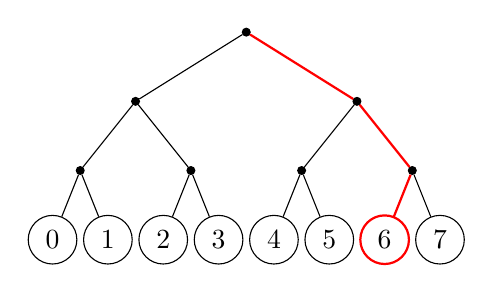
\begin{tikzpicture}
        \begin{scope} [leaf_tree_3]
            \node [style = {leaf_tree_inner_node}] {}
                child {
                    node [style = {leaf_tree_inner_node}] {}
                    child {
                        node [style = {leaf_tree_inner_node}] {}
                        child {
                            node [style = {leaf_tree_leaf}] {0}
                        }
                        child {
                            node [style = {leaf_tree_leaf}] {1}
                        }
                    }
                    child {
                        node [style = {leaf_tree_inner_node}] {}
                        child {
                            node [style = {leaf_tree_leaf}] {2}
                        }
                        child {
                            node [style = {leaf_tree_leaf}] {3}
                        }
                    }
                }
                child {
                    node [style = {leaf_tree_inner_node}] {}
                    child[black, thin] {
                        node [style = {leaf_tree_inner_node}] {}
                        child {
                            node [style = {leaf_tree_leaf}] {4}
                        }
                        child {
                            node [style = {leaf_tree_leaf}] {5}
                        }
                    }
                    child {
                        node[black, thin] [style = {leaf_tree_inner_node}] {}
                        child {
                            node [style = {leaf_tree_leaf}] {6}
                        }
                        child[black, thin] {
                            node [style = {leaf_tree_leaf}] {7}
                        }
                        edge from parent[red, thick]
                    }
                    edge from parent[red, thick]
                };
        \end{scope}
    \end{tikzpicture}}}$
    \coqinline{~> 6}
\end{center}

In this case we suppose that all arguments are valid, but we still have to return option, as we need to return something in all cases.

\begin{coq}
Fixpoint complete_binary_leaf_tree_nth {A} d il (blt : binary_leaf_tree A) : option A :=
  match il, blt with
  | [], BinaryLeafTreeLeaf x => Some x
  | 0 :: il', BinaryLeafTreeInternalNode blt'1 _ => complete_binary_leaf_tree_nth (pred d) il' blt'1
  | 1 :: il', BinaryLeafTreeInternalNode _ blt'2 => complete_binary_leaf_tree_nth (pred d) il' blt'2
  | _, _ => None
  end.
\end{coq}

Now, consider the following digital list:

\begin{center}
    $\xbraces{
        \vcenter{\hbox{\completebinaryleaftreedepththree{$0$}{$1$}{$2$}{$3$}{$4$}{$5$}{$6$}{$7$}}};
        \vcenter{\hbox{\bigvarnothing}};
        \vcenter{\hbox{\completebinaryleaftreedepthone{$8$}{$9$}}};
        \vcenter{\hbox{\completebinaryleaftreedepthzero{$10$}}}
    }$
\end{center}

To see how to extract the \coqinline{i}th element, we need to know in which it is stored at which index. Let us see on this example what we get:

\begin{center}
    \begin{tabular}{|c|c|c|}
        \hline
        \textbf{Element index} & \textbf{Tree index} & \textbf{Index in tree} \\
        \hline
        $\textcolor{red}{0}000_2$ & $\textcolor{red}{0}$ & $000_2$ \\
        $\textcolor{red}{0}001_2$ & $\textcolor{red}{0}$ & $001_2$ \\
        $\textcolor{red}{0}010_2$ & $\textcolor{red}{0}$ & $010_2$ \\
        $\textcolor{red}{0}011_2$ & $\textcolor{red}{0}$ & $011_2$ \\
        $\textcolor{red}{0}100_2$ & $\textcolor{red}{0}$ & $100_2$ \\
        $\textcolor{red}{0}101_2$ & $\textcolor{red}{0}$ & $101_2$ \\
        $\textcolor{red}{0}110_2$ & $\textcolor{red}{0}$ & $110_2$ \\
        $\textcolor{red}{0}111_2$ & $\textcolor{red}{0}$ & $111_2$ \\
        $10\textcolor{teal}{0}0_2$ & $\textcolor{teal}{2}$ & $0_2$ \\
        $10\textcolor{teal}{0}1_2$ & $\textcolor{teal}{2}$ & $1_2$ \\
        $101\textcolor{blue}{0}_2$ & $\textcolor{blue}{3}$ & $\varepsilon_2$ \\
        \hline
        $\textcolor{red}{1}0\textcolor{teal}{1}\textcolor{blue}{1}_2$ & \multicolumn{2}{|c|}{$\leftarrow$ \textbf{Count of elements in whole digital list}} \\
        \hline
    \end{tabular}
\end{center}

The crucial observation here is that the tree index is the index of the first digit in \coqinline{i} that is less than the corresponding digit of \coqinline{n}, and the index in the tree is just the rest of digits of \coqinline{i}.

So in the case $i_{d - 1} = n_{d - 1} = 0$ (that is, \coqinline{il} starts with 0 and there is no tree in this position) and in the case $i_{d - 1} = n_{d - 1} = 1$ (that is, \coqinline{il} starts with 1 and there is a tree in this position), we recurse to our tail. Otherwise, in the case $i_{d - 1} = 0$ and $n_{d - 1} = 1$ (that is, \coqinline{il} starts with 0 and there is a tree in this position), we ask this tree for its element at position defined by \coqinline{il'}. The case $i_{d - 1} = 1$ and $n_{d - 1} = 0$ is impossible on valid input.

\begin{coq}
Fixpoint digital_list_nth_inner {A} d il (dl : digital_list A) : option A :=
  match il, dl with
  | 0 :: il', DigitalListCons None dl'
  | 1 :: il', DigitalListCons (Some _) dl' => digital_list_nth_inner (pred d) il' dl'
  | 0 :: il', DigitalListCons (Some blt) dl' => complete_binary_leaf_tree_nth (pred d) il' blt
  | _, _ => None
  end.
\end{coq}

All that is left now is to check whether \coqinline{i} is in bounds (to get a functions that works on and \coqinline{i}) and to convert it into digits.

\begin{coq}
Definition digital_list_nth {A} d i (dl : digital_list A) : option A :=
  if Nat.ltb i (digital_list_length d dl)
  then digital_list_nth_inner d (to_digits d i) dl
  else None.

Definition concrete_digital_list_nth {A} i (cdl : concrete_digital_list A) : option A :=
  let '(ConcreteDigitalList d dl) := cdl in digital_list_nth d i dl.
\end{coq}

\subsection{Updating an element by its index}

The operation of replacing the \coqinline{i}th element by another \coqinline{x : A} is completely analogous to getting the \coqinline{i}th element, the only difference is that we reconstruct back the data structures with the element updated.

\begin{coq}
Fixpoint complete_binary_leaf_tree_update {A} d il x (blt : binary_leaf_tree A) :
  option (binary_leaf_tree A) :=
  match il, blt with
  | [], _ => Some (BinaryLeafTreeLeaf x)
  | 0 :: il', BinaryLeafTreeInternalNode blt'1 blt'2 =>
    option_map
      (fun blt'1_0 => BinaryLeafTreeInternalNode blt'1_0 blt'2)
      (complete_binary_leaf_tree_update (pred d) il' x blt'1)
  | 1 :: il', BinaryLeafTreeInternalNode blt'1 blt'2 =>
    option_map
      (fun blt'2_0 => BinaryLeafTreeInternalNode blt'1 blt'2_0)
      (complete_binary_leaf_tree_update (pred d) il' x blt'2)
  | _, _ => None
  end.

Fixpoint digital_list_update_inner {A} d il x (dl : digital_list A) : option (digital_list A) :=
  match il, dl with
  | 0 :: il', DigitalListCons (None as o) dl'
  | 1 :: il', DigitalListCons (Some _ as o) dl' =>
    option_map
      (DigitalListCons o)
      (digital_list_update_inner (pred d) il' x dl')
  | 0 :: il', DigitalListCons (Some blt) dl' =>
    Some (DigitalListCons (complete_binary_leaf_tree_update (pred d) il' x blt) dl')
  | _, _ => None
  end.

Definition digital_list_update {A} d i x (dl : digital_list A) : option (digital_list A) :=
  if Nat.ltb i (digital_list_length d dl)
  then digital_list_update_inner d (to_digits d i) x dl
  else None.

Definition concrete_digital_list_update {A} i x (cdl : concrete_digital_list A) :
  option (concrete_digital_list A) :=
  let '(ConcreteDigitalList d dl) := cdl in
    option_map (ConcreteDigitalList d) (digital_list_update d i x dl).
\end{coq}

\subsection{Adding an element to the end}

Adding an element \coqinline{x : A} to the end of a digital list of depth \coqinline{d} can potentially produce a carry (a complete binary leaf tree of depth \coqinline{d}) and always gives a digital list of the same depth \coqinline{d}.

If the initial digital list is of depth $0$, we output a carry with the element $x$. For example:

\begin{center}
    \coqinline{digital_list_push 0 8}
    $\xbraces{
        \vcenter{\hbox{\spacer}}
    }$
    \evaluatesto
    $\left(
        \,\vcenter{\hbox{\completebinaryleaftreedepthzero{$8$}}}\,,
        \xbraces{
            \vcenter{\hbox{\spacer}}
        }
    \right)$
\end{center}

Else, we recurse. Suppose that we did not get a carry. In this case, we just add our digit (if it exists) to the result of the recursive call. For example, if the recursive call looked like this:

\begin{center}
    \coqinline{digital_list_push 2 8}
    $\xbraces{
        \vcenter{\hbox{\completebinaryleaftreedepthone{$4$}{$5$}}};
        \vcenter{\hbox{\bigvarnothing}}
    }$
    \evaluatesto
    $\left(
        \vcenter{\hbox{\bigvarnothing}}\,,
        \xbraces{
            \vcenter{\hbox{\completebinaryleaftreedepthone{$4$}{$5$}}};
            \vcenter{\hbox{\completebinaryleaftreedepthzero{$8$}}}
        }
    \right)$
\end{center}

Then the parent execution can be the following:

\begin{center}
    \coqinline{digital_list_push 3 8}
    $\xbraces{
        \vcenter{\hbox{\completebinaryleaftreedepthtwo{$0$}{$1$}{$2$}{$3$}}};
        \vcenter{\hbox{\completebinaryleaftreedepthone{$4$}{$5$}}};
        \vcenter{\hbox{\bigvarnothing}}
    }$
    \evaluatesto
    $\left(
        \vcenter{\hbox{\bigvarnothing}}\,,
        \xbraces{
            \vcenter{\hbox{\completebinaryleaftreedepthtwo{$0$}{$1$}{$2$}{$3$}}};
            \vcenter{\hbox{\completebinaryleaftreedepthone{$4$}{$5$}}};
            \vcenter{\hbox{\completebinaryleaftreedepthzero{$8$}}}
        }
    \right)$
\end{center}

Else there was a carry. And again, the are two cases, depending on whether or not the head of the digital list contains a tree. If it does not, we just add the carry that we got in this place. For example, if the recursive call looked like this:

\begin{center}
    \coqinline{digital_list_push 2 8}
    $\xbraces{
        \vcenter{\hbox{\completebinaryleaftreedepthone{$0$}{$1$}}};
        \vcenter{\hbox{\completebinaryleaftreedepthzero{$2$}}}
    }$
    \evaluatesto
    $\left(
        \,\vcenter{\hbox{\completebinaryleaftreedepthtwo{$0$}{$1$}{$2$}{$8$}}}\,,
        \xbraces{
            \vcenter{\hbox{\bigvarnothing}};
            \vcenter{\hbox{\bigvarnothing}}
        }
    \right)$
\end{center}

Then the parent execution can be the following:

\begin{center}
    \coqinline{digital_list_push 3 8}
    $\xbraces{
        \vcenter{\hbox{\bigvarnothing}};
        \vcenter{\hbox{\completebinaryleaftreedepthone{$0$}{$1$}}};
        \vcenter{\hbox{\completebinaryleaftreedepthzero{$2$}}}
    }$
    \evaluatesto
    $\left(
        \vcenter{\hbox{\bigvarnothing}}\,,
        \xbraces{
            \vcenter{\hbox{\completebinaryleaftreedepthtwo{$0$}{$1$}{$2$}{$8$}}};
            \vcenter{\hbox{\bigvarnothing}};
            \vcenter{\hbox{\bigvarnothing}}
        }
    \right)$
\end{center}

But if the head of the list contains a tree, then we create a tree from it and the carry and return it again as a carry. For example, if the recursive call looked like this:

\begin{center}
    \coqinline{digital_list_push 1 8}
    $\xbraces{
        \vcenter{\hbox{\completebinaryleaftreedepthzero{$2$}}}
    }$
    \evaluatesto
    $\left(
        \,\vcenter{\hbox{\completebinaryleaftreedepthone{$2$}{$8$}}}\,,
        \xbraces{
            \vcenter{\hbox{\bigvarnothing}}
        }
    \right)$
\end{center}

Then the parent execution can be the following:

\begin{center}
    \coqinline{digital_list_push 2 8}
    $\xbraces{
        \vcenter{\hbox{\completebinaryleaftreedepthone{$0$}{$1$}}};
        \vcenter{\hbox{\completebinaryleaftreedepthzero{$2$}}}
    }$
    \evaluatesto
    $\left(
        \,\vcenter{\hbox{\completebinaryleaftreedepthtwo{$0$}{$1$}{$2$}{$8$}}}\,,
        \xbraces{
            \vcenter{\hbox{\bigvarnothing}};
            \vcenter{\hbox{\bigvarnothing}}
        }
    \right)$
\end{center}

We can remark an analogy with binary adders:

\begin{center}
    \begin{tabular}{|c|c||c|c|}
        \hline
        \textbf{First operand} & \textbf{Second operand} & \textbf{Carry} & \textbf{Result} \\
        \hline
        $0$ & $0$ & $0$ & $0$ \\
        $0$ & $1$ & $0$ & $1$ \\
        $1$ & $0$ & $0$ & $1$ \\
        $1$ & $1$ & $1$ & $0$ \\
        \hline
    \end{tabular}
\end{center}

\begin{coq}
Fixpoint digital_list_push {A} d x (dl : digital_list A) : option (binary_leaf_tree A) * (digital_list A) :=
  match dl with
  | DigitalListNil => (Some (BinaryLeafTreeLeaf x), DigitalListNil)
  | DigitalListCons o dl' =>
    match digital_list_push (pred d) x dl' with
    | (None, dl'0) => (None, DigitalListCons o dl'0)
    | (Some blt0, dl'0) =>
      match o with
      | None => (None, DigitalListCons (Some blt0) dl'0)
      | Some blt => (Some (BinaryLeafTreeInternalNode blt blt0), DigitalListCons None dl'0)
      end
    end
  end.
\end{coq}

To get a concrete digital list from an optional carry and the resulting digital list, we add the carry to the head of the digital list if it exists (and get a digital list of depth one more than the original), if not, then just return the digital list from the operation.

\begin{coq}
Definition concrete_digital_list_push {A} x (cdl : concrete_digital_list A) : concrete_digital_list A :=
  let '(ConcreteDigitalList d dl) := cdl in
    match digital_list_push d x dl with
    | (None, dl0) => ConcreteDigitalList d dl0
    | (Some blt0, dl0) => ConcreteDigitalList (S d) (DigitalListCons (Some blt0) dl0)
    end.
\end{coq}

\subsection{Removing an element from the end}

To remove the last element from a complete binary leaf tree, we split it into a digital list and this element. For example:

\begin{center}
    \coqinline{complete_binary_leaf_tree_pop}
    $\vcenter{\hbox{\completebinaryleaftreedepththree{$0$}{$1$}{$2$}{$3$}{$4$}{$5$}{$6$}{$7$}}}$
    \evaluatesto
    $\left(
        \xbraces{
            \vcenter{\hbox{\completebinaryleaftreedepthtwo{$0$}{$1$}{$2$}{$3$}}};
            \vcenter{\hbox{\completebinaryleaftreedepthone{$4$}{$5$}}};
            \vcenter{\hbox{\completebinaryleaftreedepthzero{$6$}}}
        },
        7
    \right)$
\end{center}

\begin{coq}
Fixpoint complete_binary_leaf_tree_pop {A} d (blt : binary_leaf_tree A) : digital_list A * A :=
  match blt with
  | BinaryLeafTreeLeaf x => (DigitalListNil, x)
  | BinaryLeafTreeInternalNode blt'1 blt'2 =>
    let '(dl', x) := complete_binary_leaf_tree_pop (pred d) blt'2 in
      (DigitalListCons (Some blt'1) dl', x)
  end.
\end{coq}

To remove the last element of a digital list, we just recurse until we are at the last existing tree, from which we remove the element from the end, and then reconstruct back the digital list, leaving unchanged all of the previous trees. For example:

\begin{center}
    \coqinline{digital_list_pop 3 8}
    $\xbraces{
        \vcenter{\hbox{\completebinaryleaftreedepthtwo{$0$}{$1$}{$2$}{$3$}}};
        \vcenter{\hbox{\completebinaryleaftreedepthone{$4$}{$5$}}};
        \vcenter{\hbox{\bigvarnothing}}
    }$
    \evaluatesto
    $\left(
        \xbraces{
            \vcenter{\hbox{\completebinaryleaftreedepthtwo{$0$}{$1$}{$2$}{$3$}}};
            \vcenter{\hbox{\bigvarnothing}};
            \vcenter{\hbox{\completebinaryleaftreedepthzero{$4$}}}
        },
        5
    \right)$
\end{center}

The only case when we return $\varnothing$ is when the original digital list does not contain trees. For example:

\begin{center}
    \coqinline{digital_list_pop 2 8}
    $\xbraces{
        \vcenter{\hbox{\bigvarnothing}};
        \vcenter{\hbox{\bigvarnothing}}
    }$
    \evaluatesto
    $\vcenter{\hbox{\bigvarnothing}}$
\end{center}

We do not try to maintain the minimum possible depth, so the head of the digital list can become empty.

\begin{coq}
Fixpoint digital_list_pop {A} d (dl : digital_list A) : option (digital_list A * A) :=
  match dl with
  | DigitalListNil => None
  | DigitalListCons o dl' =>
    match digital_list_pop (pred d) dl' with
    | None =>
      option_map
        (fun blt =>
          let '(dl'0, x) := complete_binary_leaf_tree_pop (pred d) blt in
            (DigitalListCons None dl'0, x)
        )
        o
    | Some (dl'0, x) => Some (DigitalListCons o dl'0, x)
    end
  end.

Definition concrete_digital_list_pop {A} (cdl : concrete_digital_list A) :
  option (concrete_digital_list A * A) :=
  let '(ConcreteDigitalList d dl) := cdl in
    option_map
      (fun '(dl0, x) => (ConcreteDigitalList d dl0, x))
      (digital_list_pop d dl).
\end{coq}

\pagebreak

\printbibliography

\end{document}
